\documentclass[12pt, a4paper]{article}
\usepackage{../../../myconfig} % Gọi file cấu hình từ ngoài gốc vào

% ==========================================
% BẮT ĐẦU NỘI DUNG TÀI LIỆU
% ==========================================
\begin{document}

% Truyền 3 tham số: {Nhãn cam} {Chữ to chính giữa} {Chữ ở góc phải Header}
\titlebox{Chủ đề: Hàm số}{Khảo sát hàm số bậc 3}{Hàm số: Hàm bậc 3}

\drawdashlines{30}
\newpage
\drawdashlines{25}

% --- CÂU 1 ---
\questionLinesManual{3}{1}{Đồ thị của hàm số nào dưới đây có dạng như đường cong trong hình bên?

\begin{center}
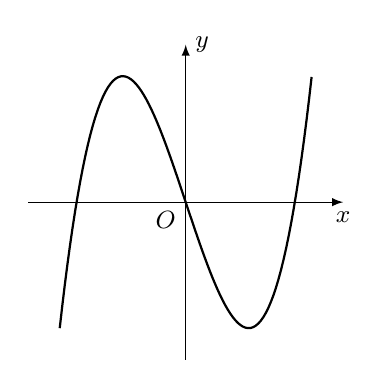
\begin{tikzpicture}[>=latex, scale=0.8]
    % Hệ trục tọa độ
    \draw[->] (-2.5,0) -- (2.5,0) node[below] {\small $x$};
    \draw[->] (0,-2.5) -- (0,2.5) node[right] {\small $y$};
    \node[below left] at (0,0) {\small $O$};
    
    % Đồ thị hàm bậc 3: y = x^3 - 3x
    \draw[thick, samples=100, domain=-2:2] 
        plot (\x, {\x*\x*\x - 3*\x});
    
\end{tikzpicture}
\end{center}

}{
    \begin{tasks}(4)
        \task \( y = x^3 - 3x \)
        \task \( y = -x^3 + 3x \)
        \task \( y = x^4 - 2x^2 \)
        \task \( y = -x^4 + 2x^2 \)
    \end{tasks}
}

\questionLinesManual{3}{2}{Đường cong hình bên là đồ thị của một trong bốn hàm số dưới đây. Hàm số đó là hàm số nào?

\begin{center}
\begin{tikzpicture}[>=latex, scale=0.8]
    % Hệ trục tọa độ
    \draw[->] (-3.5,0) -- (3.5,0) node[below] {\small $x$};
    \draw[->] (0,-2.5) -- (0,5.5) node[right] {\small $y$};
    \node[below left] at (0,0) {\small $O$};
    
    % Đồ thị hàm bậc 3: y = -x^3 + 3x + 2
    \draw[thick, samples=100, domain=-2.2:2.1] 
        plot (\x, {\x*\x*\x - 3*\x + 2});
    
  
\end{tikzpicture}
\end{center}

}{
    \begin{tasks}(4)
        \task \( y = -x^3 + 3x + 2 \)
        \task \( y = x^4 - x^2 + 1 \)
        \task \( y = x^4 + x^2 + 1 \)
        \task \( y = x^3 - 3x + 2 \)
    \end{tasks}
}

\questionLinesManual{8}{3}{Hình vẽ sau đây là đồ thị của một trong bốn hàm số cho ở các đáp án. Hỏi đó là hàm số nào?

\begin{center}
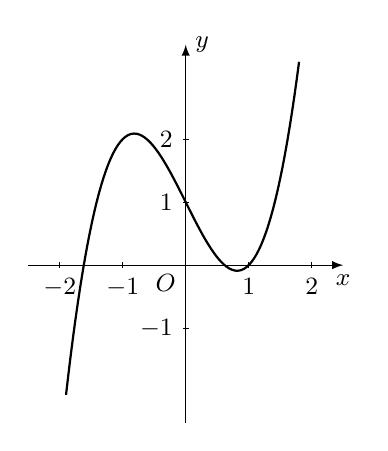
\begin{tikzpicture}[>=latex, scale=0.8]
    % Hệ trục tọa độ
    \draw[->] (-2.5,0) -- (2.5,0) node[below] {\small $x$};
    \draw[->] (0,-2.5) -- (0,3.5) node[right] {\small $y$};
    \node[below left] at (0,0) {\small $O$};
    \foreach \x in {-2,-1,1,2} {
         \draw (\x,0.05) -- (\x,-0.05)  node[below] {\small $\x$};
    }
    \foreach \y in {-1,1,2} {
          \draw (0.05,\y) -- (-0.05,\y)   node[left] {\small $\y$};
    }
    % Đồ thị hàm bậc 3: y = x^3 - 2x + 1
    \draw[thick, samples=100, domain=-1.9:1.8] 
        plot (\x, {\x*\x*\x - 2*\x + 1});
    
\end{tikzpicture}
\end{center}

}{
    \begin{tasks}(4)
        \task \( y = x^3 + 2x + 1 \)
        \task \( y = x^3 - 2x^2 + 1 \)
        \task \( y = x^3 - 2x + 1 \)
        \task \( y = -x^3 + 2x + 1 \)
    \end{tasks}
}

\questionLinesManual{8}{4}{Đồ thị sau đây là của hàm số nào?

\begin{center}
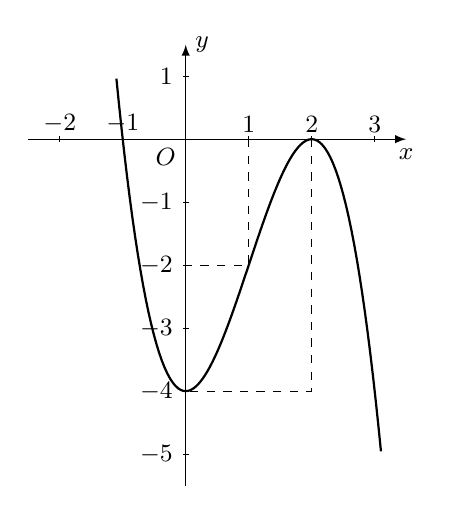
\begin{tikzpicture}[>=latex, scale=0.8]
    % Hệ trục tọa độ
    \draw[->] (-2.5,0) -- (3.5,0) node[below] {\small $x$};
    \draw[->] (0,-5.5) -- (0,1.5) node[right] {\small $y$};
    \node[below left] at (0,0) {\small $O$};
    
    % Đánh dấu các mốc
    \foreach \x in {-2,-1,1,2,3} {
         \draw (\x,0.05) -- (\x,-0.05)  node[above] {\small $\x$};
    }
    \foreach \y in {-5,-4,-3,-2,-1,1} {
          \draw (0.05,\y) -- (-0.05,\y)   node[left] {\small $\y$};
    }
    \draw[dashed] (1,0) -- (1,-2) -- (0,-2);
    \draw[dashed] (2,0) -- (2,-4) -- (0,-4);
    % Đồ thị hàm bậc 3: y = x^3 + 3x^2 - 4
    \draw[thick, samples=100, domain=-1.1:3.1] 
        plot (\x, {-\x*\x*\x + 3*\x*\x - 4});
\end{tikzpicture}
\end{center}

}{
    \begin{tasks}(4)
        \task \( y = -x^3 - 3x^2 - 4 \)
        \task \( y = x^3 + 3x^2 - 4 \)
        \task \( y = x^3 - 3x - 4 \)
        \task \( y = -x^3 + 3x^2 - 4 \)
    \end{tasks}
}

\questionLinesManual{8}{5}{Đường cong ở hình sau là đồ thị của một trong bốn hàm số dưới đây. Hàm số đó là hàm số nào?

\begin{center}
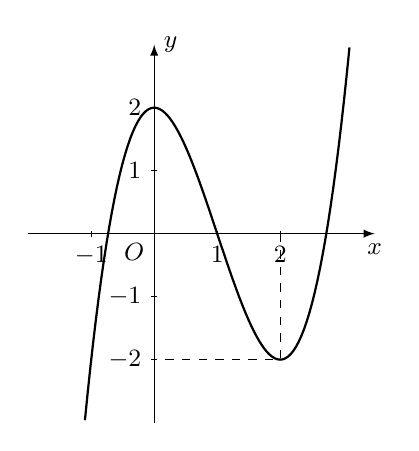
\begin{tikzpicture}[>=latex, scale=0.8]
    % Hệ trục tọa độ
    \draw[->] (-2,0) -- (3.5,0) node[below] {\small $x$};
    \draw[->] (0,-3) -- (0,3) node[right] {\small $y$};
    \node[below left] at (0,0) {\small $O$};
    
    % Đánh dấu các mốc
    \foreach \x in {-1,1,2} {
         \draw (\x,0.05) -- (\x,-0.05)  node[below] {\small $\x$};
    }
    \foreach \y in {-2,-1,1,2} {
          \draw (0.05,\y) -- (-0.05,\y)   node[left] {\small $\y$};
    }
    \draw[dashed] (2,0) -- (2,-2) -- (0,-2);
    % Đồ thị hàm bậc 3: y = x^3 - 3x + 2
    \draw[thick, samples=100, domain=-1.1:3.1] 
        plot (\x, {\x*\x*\x - 3*\x*\x + 2});
    
\end{tikzpicture}
\end{center}

}{
    \begin{tasks}(4)
        \task \( y = x^3 - 3x + 2 \)
        \task \( y = x^3 - 3x^2 + 2 \)
        \task \( y = x^3 - 6x + 2 \)
        \task \( y = -x^3 + 3x^2 + 2 \)
    \end{tasks}
}


\questionLinesManual{8}{6}{Cho hàm số bậc ba \( y = f(x) \) có đồ thị như hình vẽ. Công thức của hàm số bậc ba đã cho là:

\begin{center}
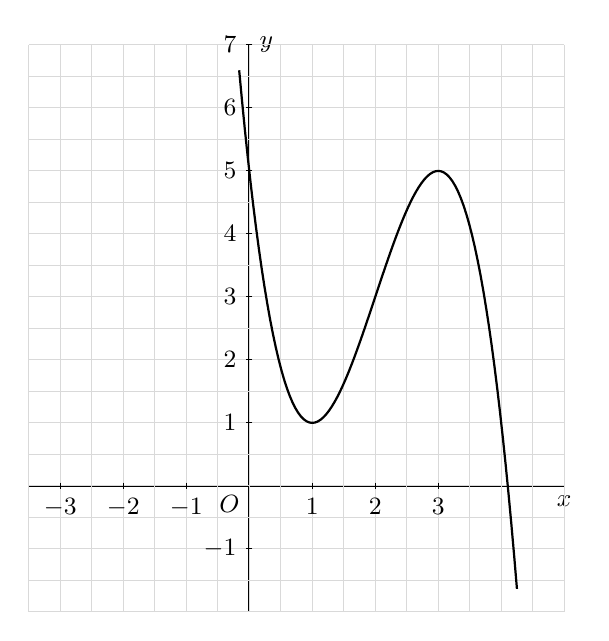
\begin{tikzpicture}[>=latex, scale=0.8]
\draw[thick] (-3.5,0) -- (5,0) node[below] {\small $x$};
    \draw[thick] (0,-2) -- (0,7) node[right] {\small $y$};
    \node[below left] at (0,0) {\small $O$};
    \draw[color=gray!30, thin, step=0.5] (-3.5,-2) grid (5,7);
    % Đánh dấu các mốc
    \foreach \x in {-3,-2,-1,1,2,3} {
        \draw (\x,0.05) -- (\x,-0.05) node[below] {\small $\x$};
    }
    \foreach \y in {-1,1,2,3,4,5,6,7} {
        \draw (0.05,\y) -- (-0.05,\y) node[left] {\small $\y$};
    }
    
    % Đồ thị hàm bậc 3: y = -x^3 + 6x^2 - 9x + 5
    \draw[thick, samples=100, domain=-0.16:4.25] 
        plot (\x, {-\x*\x*\x + 6*\x*\x - 9*\x + 5});
\end{tikzpicture}  
\end{center}

}{
    \begin{tasks}(2)
        \task \( y = x^3 - 5x + 5 \)
        \task \( y = -x^3 + 6x^2 + 9x + 5 \)
        \task \( y = -x^3 + 6x^2 - 9x + 5 \)
        \task \( y = x^3 - 2x^2 - 3x + 5 \)
    \end{tasks}
}

\questionLinesManual{8}{7}{Cho hàm số bậc ba \( y = f(x) \) có bảng biến thiên như sau:

\begin{center}

\begin{tikzpicture}
    \tkzTabInit[lgt=1.5, espcl=2.5]
    {$x$ /1, $y'$ /1, $y$ /2.5}
    {$-\infty$, $-2$, $0$, $+\infty$}
    \tkzTabLine{, +, 0, -, 0, +, }
    \tkzTabVar{-/ $-\infty$ / , +/ $2$ / , -/ $-2$ / , +/ $+\infty$ /}
\end{tikzpicture}
\end{center}

Khẳng định nào sau đây đúng?}{
    \begin{tasks}(2)
        \task \( f(x) = \dfrac{x^3}{3} + x^2 - 2 \)
        \task \( f(x) = x^3 + 3x^2 - 2 \)
        \task \( f(x) = -x^3 + 3x^2 - 2 \)
        \task \( f(x) = x^3 + 3x - 2 \)
    \end{tasks}
}

\questionLinesManual{8}{8}{Hình vẽ sau là bảng biến thiên của hàm số nào dưới đây?

\begin{center}

\begin{tikzpicture}
    \tkzTabInit[lgt=1.5, espcl=2.5]
    {$x$ /1, $y'$ /1, $y$ /2.5}
    {$-\infty$, $-1$, $1$, $+\infty$}
    \tkzTabLine{, -, 0, +, 0, -, }
    \tkzTabVar{+/ $+\infty$ / , -/ $-5$ / , +/ $3$ / , -/ $-\infty$ /}
\end{tikzpicture}
\end{center}

}{
    \begin{tasks}(4)
        \task \( y = -2x^4 + x^2 - 1 \)
        \task \( y = \dfrac{-2x + 7}{x + 3} \)
        \task \( y = -2x^2 + x - 1 \)
        \task \( y = -2x^3 + 6x - 1 \)
    \end{tasks}
}

\questionLinesManual{5}{9}{Cho hàm số bậc ba \( y = f(x) \) có đồ thị là đường cong trong hình dưới đây:

\begin{center}
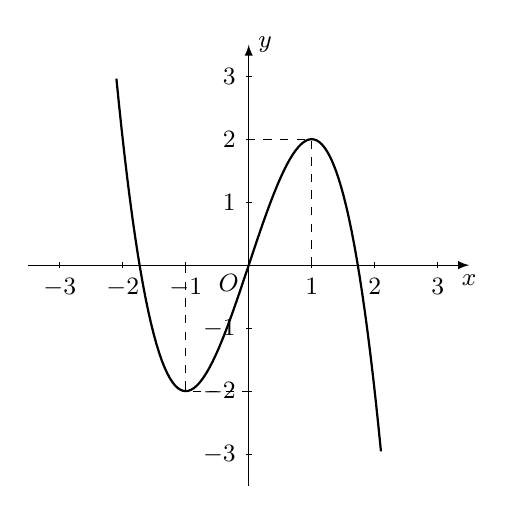
\begin{tikzpicture}[>=latex, scale=0.8]
    % Hệ trục tọa độ
    \draw[->] (-3.5,0) -- (3.5,0) node[below] {\small $x$};
    \draw[->] (0,-3.5) -- (0,3.5) node[right] {\small $y$};
    \node[below left] at (0,0) {\small $O$};
    
    % Đánh dấu các mốc
    \foreach \x in {-3,-2,-1,1,2,3} {
         \draw (\x,0.05) -- (\x,-0.05)  node[below] {\small $\x$};
    }
    \foreach \y in {-3,-2,-1,1,2,3} {
          \draw (0.05,\y) -- (-0.05,\y)   node[left] {\small $\y$};
    }
    
    % Đồ thị hàm bậc 3: y = x^3 - 3x + 1
    \draw[thick, samples=100, domain=-2.1:2.1] 
        plot (\x, {-\x*\x*\x + 3*\x});
    \draw[dashed] (1,0) -- (1,2)--(0,2);
    \draw[dashed] (-1,0) -- (-1,-2) -- (0,-2);
    
\end{tikzpicture}
\end{center}

Số nghiệm thực của phương trình \( f(x) = 3 \) là}{
    \begin{tasks}(4)
        \task $3$
        \task $0$
        \task $2$
        \task $1$
    \end{tasks}
}

\questionLinesManual{5}{10}{Cho hàm số \( y = f(x) = ax^3 + bx^2 + cx + d \) (\( a \neq 0 \)) có đồ thị như hình vẽ.

\begin{center}
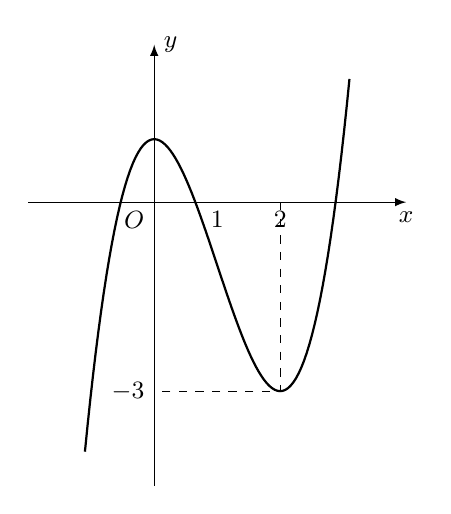
\begin{tikzpicture}[>=latex, scale=0.8]
    % Hệ trục tọa độ
    \draw[->] (-2,0) -- (4,0) node[below] {\small $x$};
    \draw[->] (0,-4.5) -- (0,2.5) node[right] {\small $y$};
    \node[below left] at (0,0) {\small $O$};
    
    
    % Đồ thị hàm bậc 3: y = x^3 - 3x
    \draw[thick, samples=100, domain=-1.1:3.1] 
        plot (\x, {\x*\x*\x - 3*\x*\x + 1});
    
    % Đánh dấu điểm cực trị
    \draw[dashed] (2,0) -- (2,-3) -- (0,-3);
    \node[below] at (1,0) {\small $1$};
    \node[below] at (2,0) {\small $2$};
    \node[left] at (0,-3) {\small $-3$};
\end{tikzpicture}
\end{center}

Số nghiệm của phương trình \( f(x) = -2 \) là}{
    \begin{tasks}(4)
        \task $2$
        \task $0$
        \task $1$
        \task $3$
    \end{tasks}
}

\questionLinesManual{5}{11}{Cho hàm số \( y = f(x) \) liên tục trên \( \mathbb{R} \) và có đồ thị như hình vẽ.

\begin{center}
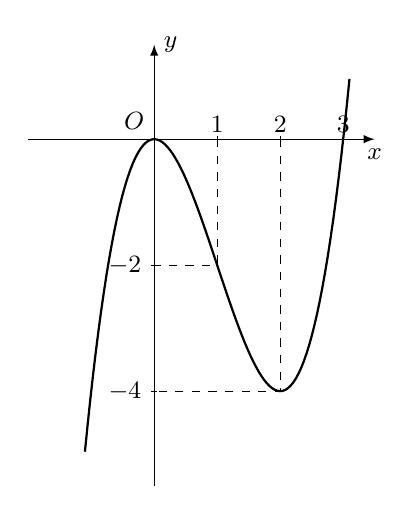
\begin{tikzpicture}[>=latex, scale=0.8]
    % Hệ trục tọa độ
    \draw[->] (-2,0) -- (3.5,0) node[below] {\small $x$};
    \draw[->] (0,-5.5) -- (0,1.5) node[right] {\small $y$};
    \node[above left] at (0,0) {\small $O$};
    
    % Đánh dấu các mốc
    \foreach \x in {1,2,3} {
         \draw (\x,0.05) -- (\x,-0.05)  node[above] {\small $\x$};
    }
    \foreach \y in {-4,-2} {
          \draw (0.05,\y) -- (-0.05,\y)   node[left] {\small $\y$};
    }
    
    % Đồ thị hàm bậc 3: y = x^3 - 3x
    \draw[thick, samples=100, domain=-1.1:3.1] 
        plot (\x, {\x*\x*\x - 3*\x*\x});
    
    % Đánh dấu điểm cực trị
    \draw[dashed] (2,0) -- (2,-4) -- (0,-4);
    \draw[dashed] (1,0) -- (1,-2)-- (0,-2);
    
    
\end{tikzpicture}
\end{center}

Phương trình \( f(x) = 0 \) có bao nhiêu nghiệm thực phân biệt?}{
    \begin{tasks}(4)
        \task $2$
        \task $1$
        \task $3$
        \task $0$
    \end{tasks}
}

\newpage
\drawdashlines{25}

\questionLinesManual{8}{12}{Cho hàm số \( y = ax^3 + 3x - d \) (\( a, d \in \mathbb{R} \)) có đồ thị là đường cong trong hình vẽ.

\begin{center}
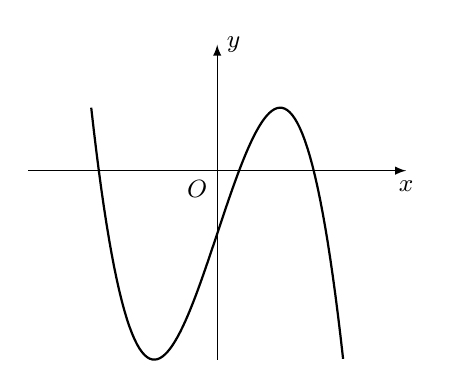
\begin{tikzpicture}[>=latex, scale=0.8]
    % Hệ trục tọa độ
    \draw[->] (-3,0) -- (3,0) node[below] {\small $x$};
    \draw[->] (0,-3) -- (0,2) node[right] {\small $y$};
    \node[below left] at (0,0) {\small $O$};
    
    
    % Đồ thị hàm bậc 3: y = -x^3 + 3x + 2
    \draw[thick, samples=100, domain=-2:2] 
        plot (\x, {-\x*\x*\x + 3*\x -1});
\end{tikzpicture}
\end{center}

Khẳng định nào dưới đây đúng?}{
    \begin{tasks}(4)
        \task \( a < 0, d > 0 \)
        \task \( a < 0, d < 0 \)
        \task \( a > 0, d < 0 \)
        \task \( a > 0, d > 0 \)
    \end{tasks}
}

\questionLinesManual{8}{13}{Cho hàm số \( y = ax^3 + bx^2 + cx + d \) (\( a, b, c, d \in \mathbb{R} \)) có đồ thị là đường cong trong hình bên. Có bao nhiêu số dương trong các số \( a, b, c, d \)?

\begin{center}

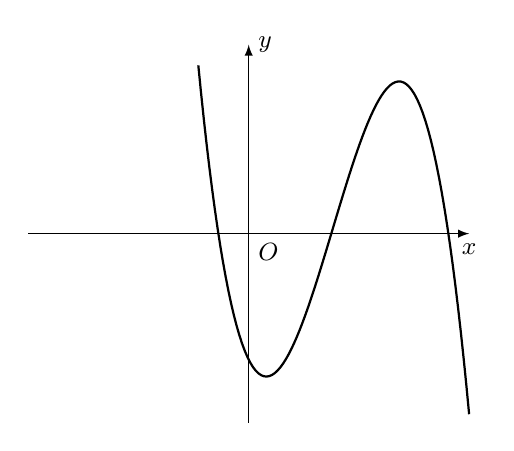
\begin{tikzpicture}[>=latex, scale=0.8]
    % Hệ trục tọa độ
    \draw[->] (-3.5,0) -- (3.5,0) node[below] {\small $x$};
    \draw[->] (0,-3) -- (0,3) node[right] {\small $y$};
    \node[below right] at (0,0) {\small $O$};
    
   
    % Đồ thị hàm bậc 3: y = x^3 - 3x
    \draw[thick, samples=100, domain=-0.8:3.5] 
        plot (\x, {-\x*\x*\x+4*\x*\x -2*\x -2});
  
\end{tikzpicture}
\end{center}

}

\questionLinesManual{5}{14}{Cho hàm số \( y = ax^3 + bx^2 + cx + d \) (\( a, b, c, d \in \mathbb{R} \)) có đồ thị là đường cong trong hình bên. Có bao nhiêu số dương trong các hệ số \( a, b, c, d \)?

\begin{center}
\begin{tikzpicture}[>=latex, scale=0.8]
    % Hệ trục tọa độ
    \draw[->] (-2,0) -- (5,0) node[below] {\small $x$};
    \draw[->] (0,-3) -- (0,5) node[right] {\small $y$};
    \node[below right] at (0,0) {\small $O$};
    
   
    % Đồ thị hàm bậc 3: y = x^3 - 3x
    \draw[thick, samples=100, domain=-0.35:4.35] 
        plot (\x, {-\x*\x*\x+6*\x*\x -8*\x +1});
  
\end{tikzpicture}
\end{center}

}

\questionLinesManual{5}{15}{Cho hàm số \( y = ax^3 + bx^2 + cx + d \) (\( a, b, c, d \in \mathbb{R} \)) có đồ thị là đường cong trong hình bên. Có bao nhiêu số dương trong các số \( a, b, c, d \)?

\begin{center}
\begin{tikzpicture}[>=latex, scale=0.8]
    % Hệ trục tọa độ
    \draw[->] (-6,0) -- (2,0) node[below] {\small $x$};
    \draw[->] (0,-3) -- (0,5) node[right] {\small $y$};
    \node[below right] at (0,0) {\small $O$};
    
   
    % Đồ thị hàm bậc 3: y = x^3 - 3x
    \draw[thick, samples=100, domain=-4.5:1.2] 
        plot (\x, {-0.5*(\x+4)*(\x+2)*(\x-1)});
  
\end{tikzpicture}
\end{center}

}

\questionLinesManual{8}{16}{Cho hàm số \( y = ax^3 + bx^2 + cx + d \) có đồ thị như hình bên. Trong các mệnh đề sau mệnh đề nào đúng?

\begin{center}
\begin{tikzpicture}[>=latex, scale=0.8]
    % Hệ trục tọa độ
    \draw[->] (-2,0) -- (5,0) node[below] {\small $x$};
    \draw[->] (0,-5) -- (0,2) node[right] {\small $y$};
    \node[below right] at (0,0) {\small $O$};
    
   
    % Đồ thị hàm bậc 3: y = x^3 - 3x
    \draw[thick, samples=100, domain=-1.8:4.2] 
        plot (\x, {0.4*(\x+1)*(\x-0.6)*(\x-4)});
  
\end{tikzpicture}
\end{center}

}{
    \begin{tasks}(2)
        \task \( ab < 0, bc > 0, cd < 0 \)
        \task \( ab < 0, bc < 0, cd > 0 \)
        \task \( ab > 0, bc > 0, cd < 0 \)
        \task \( ab > 0, bc > 0, cd > 0 \)
    \end{tasks}
}




\questionLinesManual{8}{17}{Cho hàm số \( f(x) = ax^3 + bx^2 + cx + d \) (\( a, b, c, d \in \mathbb{R} \)) có bảng biến thiên như sau:

\begin{center}

\begin{tikzpicture}
    \tkzTabInit[lgt=1.5, espcl=2.5]
    {$x$ /1, $f'(x)$ /1, $f(x)$ /2.5}
    {$-\infty$, $-2$, $0$, $+\infty$}
    \tkzTabLine{, +, 0, -, 0, +, }
    \tkzTabVar{-/ $-\infty$ / , +/ $2$ / , -/ $1$ / , +/ $+\infty$ /}
\end{tikzpicture}
\end{center}

Có bao nhiêu số dương trong các số \( a, b, c, d \)?}

\questionLinesManual{5}{18}{Cho hàm số \( f(x) = ax^3 + bx^2 + cx + d \) (\( a, b, c, d \in \mathbb{R} \)) có bảng biến thiên như sau:

\begin{center}

\begin{tikzpicture}
    \tkzTabInit[lgt=1.5, espcl=2.5]
    {$x$ /1, $f'(x)$ /1, $f(x)$ /2.5}
    {$-\infty$, $0$, $4$, $+\infty$}
    \tkzTabLine{, +, 0, -, 0, +, }
    \tkzTabVar{-/ $-\infty$ / , +/ $3$ / , -/ $-5$ / , +/ $+\infty$ /}
\end{tikzpicture}
\end{center}

Có bao nhiêu số dương trong các số \( a, b, c, d \)?}

\questionLinesManual{5}{19}{Cho hàm số \( f(x) = ax^3 + bx^2 + cx + d \) (\( a, b, c, d \in \mathbb{R} \)) có bảng biến thiên như sau:

\begin{center}

\begin{tikzpicture}
    \tkzTabInit[lgt=1.5, espcl=2.5]
    {$x$ /1, $f'(x)$ /1, $f(x)$ /2.5}
    {$-\infty$, $0$, $4$, $+\infty$}
    \tkzTabLine{, +, 0, -, 0, +, }
    \tkzTabVar{-/ $-\infty$ / , +/ $-1$ / , -/ $-5$ / , +/ $+\infty$ /}
\end{tikzpicture}
\end{center}

Có bao nhiêu số dương trong các số \( a, b, c, d \)?}

\newpage
\drawdashlines{25}

\questionLinesManual{10}{20}{Phương trình tiếp tuyến của đồ thị hàm số \( y = x^3 - 3x \) tại điểm có hoành độ bằng 2 là}

\questionLinesManual{10}{21}{Tiếp tuyến của đồ thị hàm số \( y = x^3 - 1 \) tại điểm \( M(1; 0) \) có phương trình là?}

\questionLinesManual{10}{22}{Cho hàm số \( y = x^3 - 3x \) có đồ thị \( (C) \). Có bao nhiêu điểm thuộc đồ thị \( (C) \) sao cho tiếp tuyến của đồ thị \( (C) \) tại các điểm đó song song với đường thẳng \( y = 9x + 16 \)?}

\questionLinesManual{10}{23}{Cho hàm số \( y = 2x^2 + 3x - 1 \) có đồ thị \( C \). Tiếp tuyến của \( C \) vuông góc với đường thẳng \( y = x \) có phương trình là}

\questionLinesManual{10}{24}{Số giao điểm của đồ thị hàm số \( y = x^3 - 3x^2 + 2x \) với trục \( Ox \) là}

\questionLinesManual{10}{25}{Số giao điểm của đồ thị hàm số \( y = x^3 + 3x^2 \) và đồ thị hàm số \( y = 3x^2 + 3x \) là}

\end{document}
